%==============================================================================
% Presentatie Bachelorproef – Murat Bugdayci
% Compileer met: xelatex presentatie.tex
%==============================================================================
\documentclass[aspectratio=169]{beamer}

\usetheme{hogent}

\usepackage{booktabs}
\usepackage{tikz}
\usetikzlibrary{positioning}
\usepackage{graphicx}

\graphicspath{{../bachproef/images/}{graphics/}}

%--- Metadata ----------------------------------------------------------------
\title{Competentieframework voor z/OS System Administrator en System Programmeur}
\subtitle{Level 1 \& Level 2}
\author{Murat Bugdayci \\ Promotor: Dhr.\ L.\ Blondeel Co-promotor: Dhr.\ J.\ E.\ Kok (ABN AMRO)}
\institute{Hogeschool Gent}
\date{Academiejaar 2025--2026}

%=============================================================================
\begin{document}
%=============================================================================

\begin{frame}
  \titlepage
\end{frame}

\begin{frame}{Agenda}
  \tableofcontents
\end{frame}

%=============================================================================
\section{Probleemstelling}
%=============================================================================

\begin{frame}{Probleemstelling}
  \begin{columns}
    \column{0.55\textwidth}
      \begin{itemize}
        \item IBM z/OS verwerkt \textbf{>70\%} van wereldwijde bedrijfskritische transacties
        \item \textbf{Structureel personeelstekort}: vergrijzing + massale uitstroom ervaren professionals
        \item Onderwijsinstellingen besteden \textbf{nauwelijks aandacht} aan mainframe-technologie
        \item Bestaande frameworks (SFIA, e-CF) zijn te algemeen voor z/OS
      \end{itemize}
    \column{0.42\textwidth}
      \begin{block}{Onderzoeksvraag}
        Welke competenties vereist een z/OS SysAdmin / SysProg, en hoe worden deze georganiseerd in een framework toepasbaar binnen een onderwijscontext?
      \end{block}
  \end{columns}
\end{frame}

%=============================================================================
\section{Methodologie}
%=============================================================================

\begin{frame}{Methodologie}
  \begin{center}
  \begin{tikzpicture}[
    node distance=0.6cm,
    box/.style={rectangle, draw, rounded corners=4pt,
                text centered, text width=2.6cm,
                minimum height=1.2cm, fill=hggrey!40, font=\small}
  ]
    \node[box] (lit) {Literatuur-\\studie};
    \node[box, right=of lit] (int) {Semi-ge-\\structureerde\\interviews};
    \node[box, right=of int] (dev) {Ontwikkeling\\framework\\+ PoC};
    \node[box, right=of dev] (val) {Validatie};
    \draw[->] (lit) -- (int);
    \draw[->] (int) -- (dev);
    \draw[->] (dev) -- (val);
  \end{tikzpicture}
  \end{center}

  \vspace{0.4em}
  \begin{columns}
    \column{0.48\textwidth}
      \textbf{Literatuurstudie}
      \begin{itemize}
        \item SFIA, e-CF, IBM Z Competency Framework
        \item z/OS-technologiestack
        \item Mainframe-onderwijs
      \end{itemize}
    \column{0.48\textwidth}
      \textbf{Interviews} bij 7 organisaties:
      \begin{itemize}
        \item ABN AMRO, Euroclear, KBC
        \item Halkbank, Isbank
        \item Planet NL, Broadcom
        \item Junior én senior professionals
      \end{itemize}
  \end{columns}
\end{frame}

%=============================================================================
\section{Het Competentieframework}
%=============================================================================

\begin{frame}{Het Competentieframework – Overzicht}
  \begin{center}
  \begin{tabular}{ll}
    \toprule
    \multicolumn{2}{c}{\textbf{Technische Domeinen (T1--T8)}} \\
    \midrule
    T1: Platform Fundamentals       & T5: Batch Processing \& JCL \\
    T2: Hardware \& Virtualization  & T6: Automation \& Scripting (REXX) \\
    T3: Storage \& Data Management  & T7: Subsystems \& Middleware \\
    T4: System Operations \& Tools  & T8: Networking \& Security \\
    \midrule
    \multicolumn{2}{c}{\textbf{Professionele Domeinen (P1--P4)}} \\
    \midrule
    P1: Communicatie \& Samenwerking         & P3: Change Management \\
    P2: Probleemoplossing \& Krit.\ Denken   & P4: Professionele Ontwikkeling \\
    \bottomrule
  \end{tabular}
  \end{center}
  \vspace{0.4em}
  \centering\textit{Level 1: Basis \quad $\longrightarrow$ \quad Level 2: Gevorderd}
\end{frame}

\begin{frame}{Technische Prioriteiten volgens Interviews}
  \begin{columns}
    \column{0.5\textwidth}
      \textbf{Meest kritisch voor starters:}
      \begin{enumerate}
        \item JCL (JOB, EXEC, DD, utilities)
        \item TSO/ISPF navigatie
        \item SDSF (job monitoring \& output)
        \item REXX scripting
        \item RACF basisconcepten
      \end{enumerate}
    \column{0.47\textwidth}
      \begin{alertblock}{Belangrijke bevinding}
        De grens tussen \textbf{SysAdmin} en \textbf{SysProg} is in de praktijk niet eenduidig en varieert per organisatie. \\[0.5em]
        $\Rightarrow$ Geïntegreerd framework voor beide rollen noodzakelijk.
      \end{alertblock}
  \end{columns}
\end{frame}

%=============================================================================
\section{Proof-of-Concept Webapplicatie}
%=============================================================================

\begin{frame}{Proof-of-Concept Webapplicatie}
  \begin{columns}
    \column{0.42\textwidth}
      \textbf{Wat?} Statische webapplicatie via GitHub Pages \\[0.5em]
      \textbf{Elke competentiekaart bevat:}
      \begin{itemize}
        \item Theoretische uitleg
        \item MCQ-vragen
        \item Praktijkopdrachten
      \end{itemize}
      \vspace{0.5em}
      \begin{tabular}{ccc}
        \toprule
        \textbf{25} & \textbf{232} & \textbf{61} \\
        topics & MCQ & taken \\
        \bottomrule
      \end{tabular}
    \column{0.55\textwidth}
      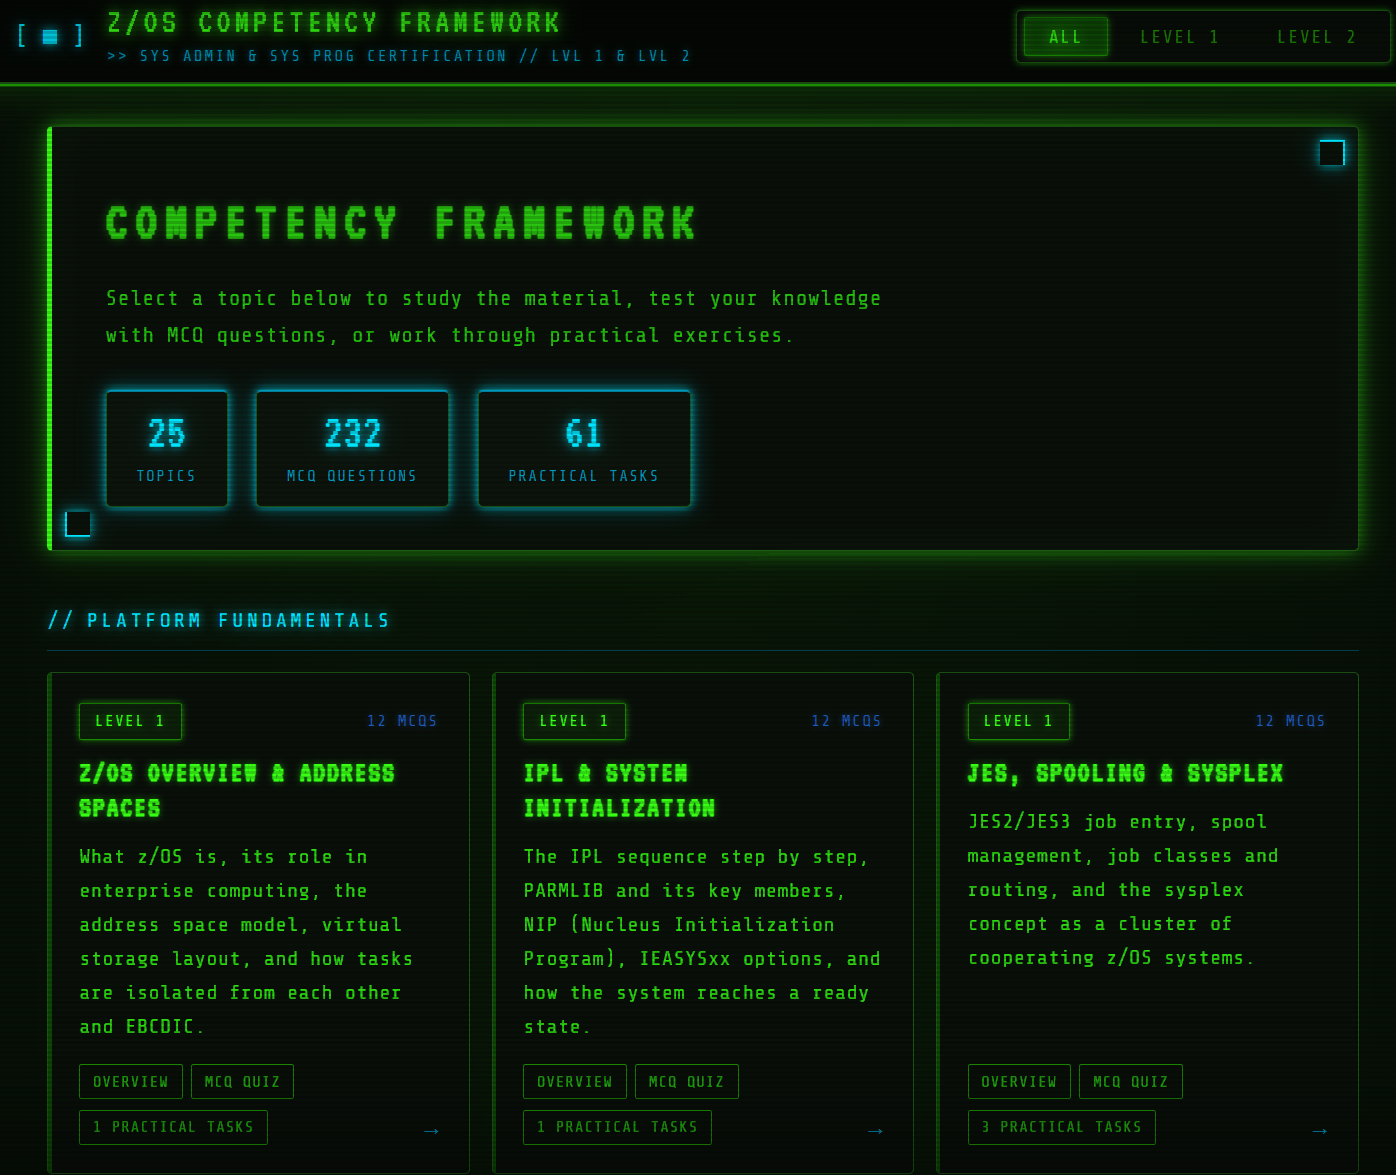
\includegraphics[width=\linewidth]{bachproef6}
  \end{columns}
\end{frame}

\begin{frame}{Demo – IEBGENER \& VSAM in de PoC}
  \begin{columns}
    \column{0.48\textwidth}
      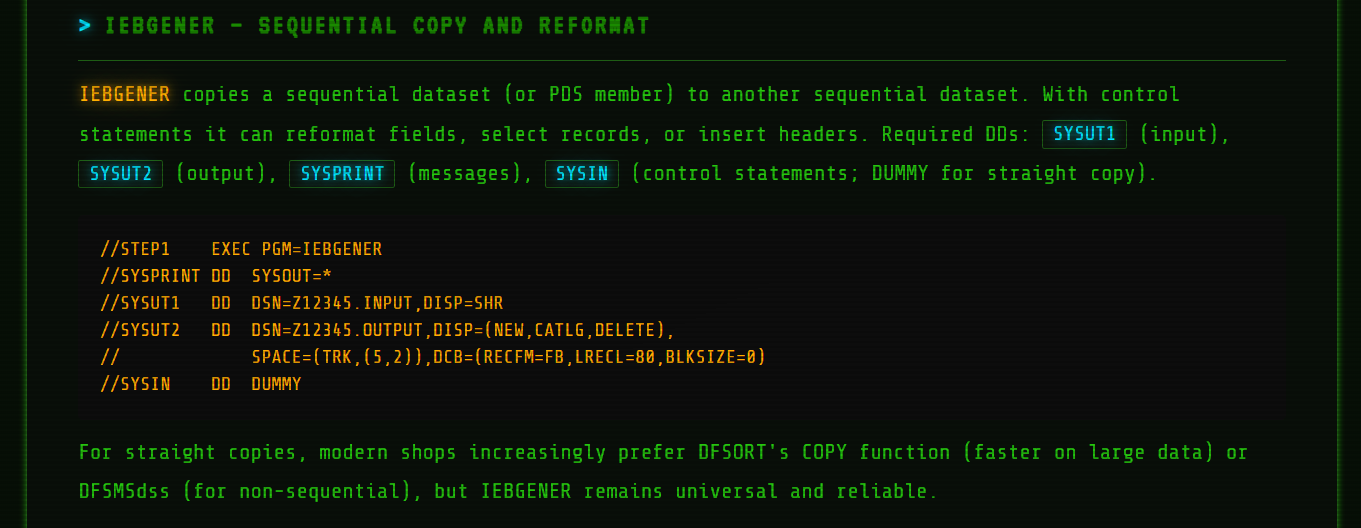
\includegraphics[width=\linewidth]{BACHPROEFGENER}
      \vspace{0.2em}
      \centering\small T5: IEBGENER utility
    \column{0.48\textwidth}
      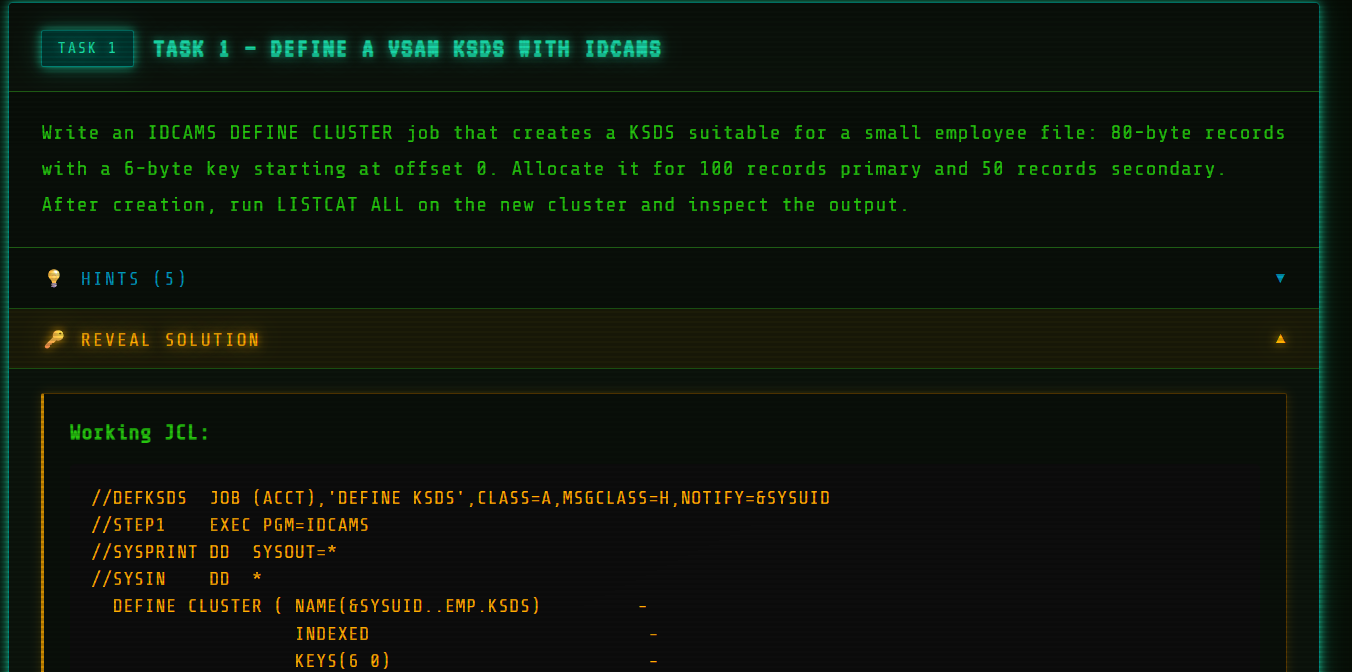
\includegraphics[width=\linewidth]{BACHPROEFVSAM}
      \vspace{0.2em}
      \centering\small T3: VSAM KSDS praktijktaak
  \end{columns}
\end{frame}

%=============================================================================
\section{Conclusies}
%=============================================================================

\begin{frame}{Conclusies}
  \begin{itemize}
    \item \textbf{Rolvervaging:} SysAdmin en SysProg overlappen sterk in de praktijk — geïntegreerd framework is noodzakelijk
    \item \textbf{Technische kern:} JCL, TSO/ISPF, SDSF en REXX zijn universeel kritisch voor starters
    \item \textbf{Soft skills:} Even belangrijk als technische kennis (communicatie, probleemoplossing, documentatie)
    \item \textbf{Unieke bijdrage:} Specifieker dan SFIA/e-CF, rechtstreeks gebaseerd op industrievalidatie
    \item \textbf{PoC als aanzet:} De webapplicatie toont de haalbaarheid van het framework in een digitale leeromgeving
  \end{itemize}
\end{frame}

%=============================================================================
\section{Beperkingen \& Toekomstig Onderzoek}
%=============================================================================

\begin{frame}{Beperkingen \& Toekomstig Onderzoek}
  \begin{columns}
    \column{0.48\textwidth}
      \textbf{Beperkingen}
      \begin{itemize}
        \item Beperkt aantal interviews — generaliseerbaarheid niet volledig gegarandeerd
        \item Geen formele validatieronde van het framework met onderwijsexperts
        \item PoC is geen productieapplicatie (geen gebruikersbeheer, geen voortgangsregistratie)
      \end{itemize}
    \column{0.48\textwidth}
      \textbf{Aanbevelingen}
      \begin{itemize}
        \item Uitbreiding naar Level 3 (Expert)
        \item Grootschalige validatie in de Benelux
        \item PoC doorontwikkelen met gesimuleerde z/OS-omgeving (IBM zXplore)
        \item Integratie in curricula via samenwerking onderwijs--industrie
      \end{itemize}
  \end{columns}
\end{frame}

%--- Vragen ------------------------------------------------------------------
\begin{frame}
  \begin{center}
    \vspace{1em}
    {\Huge \textbf{Vragen?}} \\[1.5em]
    \textit{Murat Bugdayci} \\[0.3em]
    murat.bugdayci@student.hogent.be \\[0.5em]
    \small\url{https://github.com/muratbugdayc/2026bachelorproefMuratBugdayci}
  \end{center}
\end{frame}

\end{document}
